%%%%%%%%%%%%%%%%%%%%%%%%%%%%%%%%%%%%%%%%%%%%%%%%%%%%%%%%%%%%%%%%%%%%%%%%%%%%
% AGUtmpl.tex: this template file is for articles formatted with LaTeX2e,
% Modified December 2018
%
% This template includes commands and instructions
% given in the order necessary to produce a final output that will
% satisfy AGU requirements.
%
% FOR FIGURES, DO NOT USE \psfrag
%
%%%%%%%%%%%%%%%%%%%%%%%%%%%%%%%%%%%%%%%%%%%%%%%%%%%%%%%%%%%%%%%%%%%%%%%%%%%%
%
% IMPORTANT NOTE:
%
% SUPPORTING INFORMATION DOCUMENTATION IS NOT COPYEDITED BEFORE PUBLICATION.
%
%
%
%%%%%%%%%%%%%%%%%%%%%%%%%%%%%%%%%%%%%%%%%%%%%%%%%%%%%%%%%%%%%%%%%%%%%%%%%%%%
%
% Step 1: Set the \documentclass
%
%
% PLEASE USE THE DRAFT OPTION TO SUBMIT YOUR PAPERS.
% The draft option produces double spaced output.
%
% Choose the journal abbreviation for the journal you are
% submitting to:

% jgrga JOURNAL OF GEOPHYSICAL RESEARCH (use for all of them)
% gbc   GLOBAL BIOCHEMICAL CYCLES
% grl   GEOPHYSICAL RESEARCH LETTERS
% pal   PALEOCEANOGRAPHY
% ras   RADIO SCIENCE
% rog   REVIEWS OF GEOPHYSICS
% tec   TECTONICS
% wrr   WATER RESOURCES RESEARCH
% gc    GEOCHEMISTRY, GEOPHYSICS, GEOSYSTEMS
% sw    SPACE WEATHER
% ms    JAMES
% ef    EARTH'S FUTURE
%
%
%
% (If you are submitting to a journal other than jgrga,
% substitute the initials of the journal for "jgrga" below.)

\documentclass[draft,jgrga]{agutexSI2019}

%%%%%%%%%%%%%%%%%%%%%%%%%%%%%%%%%%%%%%%%%%%%%%%%%%%%%%%%%%%%%%%%%%%%%%%%%
%
%  SUPPORTING INFORMATION TEMPLATE
%
%% ------------------------------------------------------------------------ %%
%
%
%Please use this template when formatting and submitting your Supporting Information.

%This template serves as both a “table of contents” for the supporting information for your article and as a summary of files.
%
%
%OVERVIEW
%
%Please note that all supporting information will be peer reviewed with your manuscript. It will not be copyedited if the paper is accepted.
%In general, the purpose of the supporting information is to enable authors to provide and archive auxiliary information such as data tables, method information, figures, video, or computer software, in digital formats so that other scientists can use it.
%The key criteria are that the data:
% 1. supplement the main scientific conclusions of the paper but are not essential to the conclusions (with the exception of
%    including %data so the experiment can be reproducible);
% 2. are likely to be usable or used by other scientists working in the field;
% 3. are described with sufficient precision that other scientists can understand them, and
% 4. are not exe files.
%
%USING THIS TEMPLATE
%
%***All references should be included in the reference list of the main paper so that they can be indexed, linked, and counted as citations.  The reference section does not count toward length limits.
%
%All Supporting text and figures should be included in this document. Insert supporting information content into each appropriate section of the template. To add additional captions, simply copy and paste each sample as needed.

%Tables may be included, but can also be uploaded separately, especially if they are larger than 1 page, or if necessary for retaining table formatting. Data sets, large tables, movie files, and audio files should be uploaded separately. Include their captions in this document and list the file name with the caption. You will be prompted to upload these files on the Upload Files tab during the submission process, using file type “Supporting Information (SI)”

%IMPORTANT NOTE ON FIGURES AND TABLES
% Placeholders for figures and tables appear after the \end{article} command, after references.
% DO NOT USE \psfrag or \subfigure commands.
%
 \usepackage{graphicx}
%
%  Uncomment the following command to allow illustrations to print
%   when using Draft:
 \setkeys{Gin}{draft=false}
%
% You may need to use one of these options for graphicx depending on the driver program you are using. 
%
% [xdvi], [dvipdf], [dvipsone], [dviwindo], [emtex], [dviwin],
% [pctexps],  [pctexwin],  [pctexhp],  [pctex32], [truetex], [tcidvi],
% [oztex], [textures]
%
%
%% ------------------------------------------------------------------------ %%
%
%  ENTER PREAMBLE
%
%% ------------------------------------------------------------------------ %%

% Author names in capital letters:
%\authorrunninghead{BALES ET AL.}

% Shorter version of title entered in capital letters:
%\titlerunninghead{SHORT TITLE}

%Corresponding author mailing address and e-mail address:
%\authoraddr{Corresponding author: A. B. Smith,
%Department of Hydrology and Water Resources, University of
%Arizona, Harshbarger Building 11, Tucson, AZ 85721, USA.
%(a.b.smith@hwr.arizona.edu)}

\begin{document}

%% ------------------------------------------------------------------------ %%
%
%  TITLE
%
%% ------------------------------------------------------------------------ %%

%\includegraphics{agu_pubart-white_reduced.eps}


\title{Supporting Information for "A Trajectory-based Method for Estimating the Contribution of Landfalling Atmospheric Rivers to Top-Decile Precipitation across Colorado"}
%
% e.g., \title{Supporting Information for "Terrestrial ring current:
% Origin, formation, and decay $\alpha\beta\Gamma\Delta$"}
%
%DOI: 10.1002/%insert paper number here%

%% ------------------------------------------------------------------------ %%
%
%  AUTHORS AND AFFILIATIONS
%
%% ------------------------------------------------------------------------ %%


% List authors by first name or initial followed by last name and
% separated by commas. Use \affil{} to number affiliations, and
% \thanks{} for author notes.
% Additional author notes should be indicated with \thanks{} (for
% example, for current addresses).

% Example: \authors{A. B. Author\affil{1}\thanks{Current address, Antartica}, B. C. Author\affil{2,3}, and D. E.
% Author\affil{3,4}\thanks{Also funded by Monsanto.}}

\authors{Deanna Nash\affil{1}, Jonathan J. Rutz\affil{1}, Jason Cordeira \affil{1}, F. Martin Ralph \affil{1}, Kris Sanders \affil{2}, Erin Walter \affil{2}}


% \affiliation{1}{First Affiliation}
% \affiliation{2}{Second Affiliation}
% \affiliation{3}{Third Affiliation}
% \affiliation{4}{Fourth Affiliation}

% \affiliation{=number=}{=Affiliation Address=}
\affiliation{1}{Center for Western Weather and Water Extremes, Scripps Institute of Oceanography, University of California San Diego, California}
\affiliation{2}{National Weather Service, Weather Forecast Office, Grand Junction, Colorado}
%(repeat as many times as is necessary)





%% ------------------------------------------------------------------------ %%
%
%  BEGIN ARTICLE
%
%% ------------------------------------------------------------------------ %%

% The body of the article must start with a \begin{article} command
%
% \end{article} must follow the references section, before the figures
%  and tables.

% \begin{article}

%% ------------------------------------------------------------------------ %%
%
%  TEXT
%
%% ------------------------------------------------------------------------ %%



\noindent\textbf{Contents of this file}
%%%Remove or add items as needed%%%
\begin{enumerate}
% \item Text S1 to Sx
\item Figures S1 to Sx
% \item Tables S1 to Sx
%if Tables are larger than 1 page, upload as separate excel file
\end{enumerate}
% \noindent\textbf{Additional Supporting Information (Files uploaded separately)}
% \begin{enumerate}
% \item Captions for Datasets S1 to Sx
% \item Captions for large Tables S1 to Sx (if larger than 1 page, upload as separate excel file)
% \item Captions for Movies S1 to Sx
% \item Captions for Audio S1 to Sx
% \end{enumerate}

% \noindent\textbf{Introduction}
%Type or paste your text here. The introduction gives a brief overview of the supporting information. You should include information %about as many of the following as possible (when appropriate):
% 1. a general overview of the kind of data files;
% 2. information about when and how the data were collected or created;
% 3. a general description of processing steps used;
% 4. any known imperfections or anomalies in the data.

%\clearpage

\begin{figure}
\noindent\includegraphics[width=\textwidth]{figS2.png}
\caption{(a) The backwards trajectories for all Colorado subbasins that fall within the Colorado region (black contour) for the months of December to February from 2000 to 2023 that were associated with an AR defined by the ERA5 AR Scale (Ralph et al., 2019) when the trajectory crossed the coast. (b) Same as (a) but for the Rio Grande region. (c) Same as (a) but for the South Platte region. (d) Same as (a) but for the Arkansas region. (e) Same as (a) but for the months of March to May. (f) Same as (e) but for the Rio Grande region. (g) Same as (e) but for the South Platte region. (h) Same as (e) but for the Arkansas region. (i) Same as (a) but for the months of June to August. (j) Same as (i) but for the Rio Grande region. (k) Same as (i) but for the South Platte region. (l) Same as (i) but for the Arkansas region. (m) Same as (a) but for the months of September to October. (n) Same as (m) but for the Rio Grande region. (o) Same as (m) but for the South Platte region. (p) Same as (m) but for the Arkansas region.}
\label{fig:supp:spaghetti_ssn}
\end{figure}

\begin{figure}
\noindent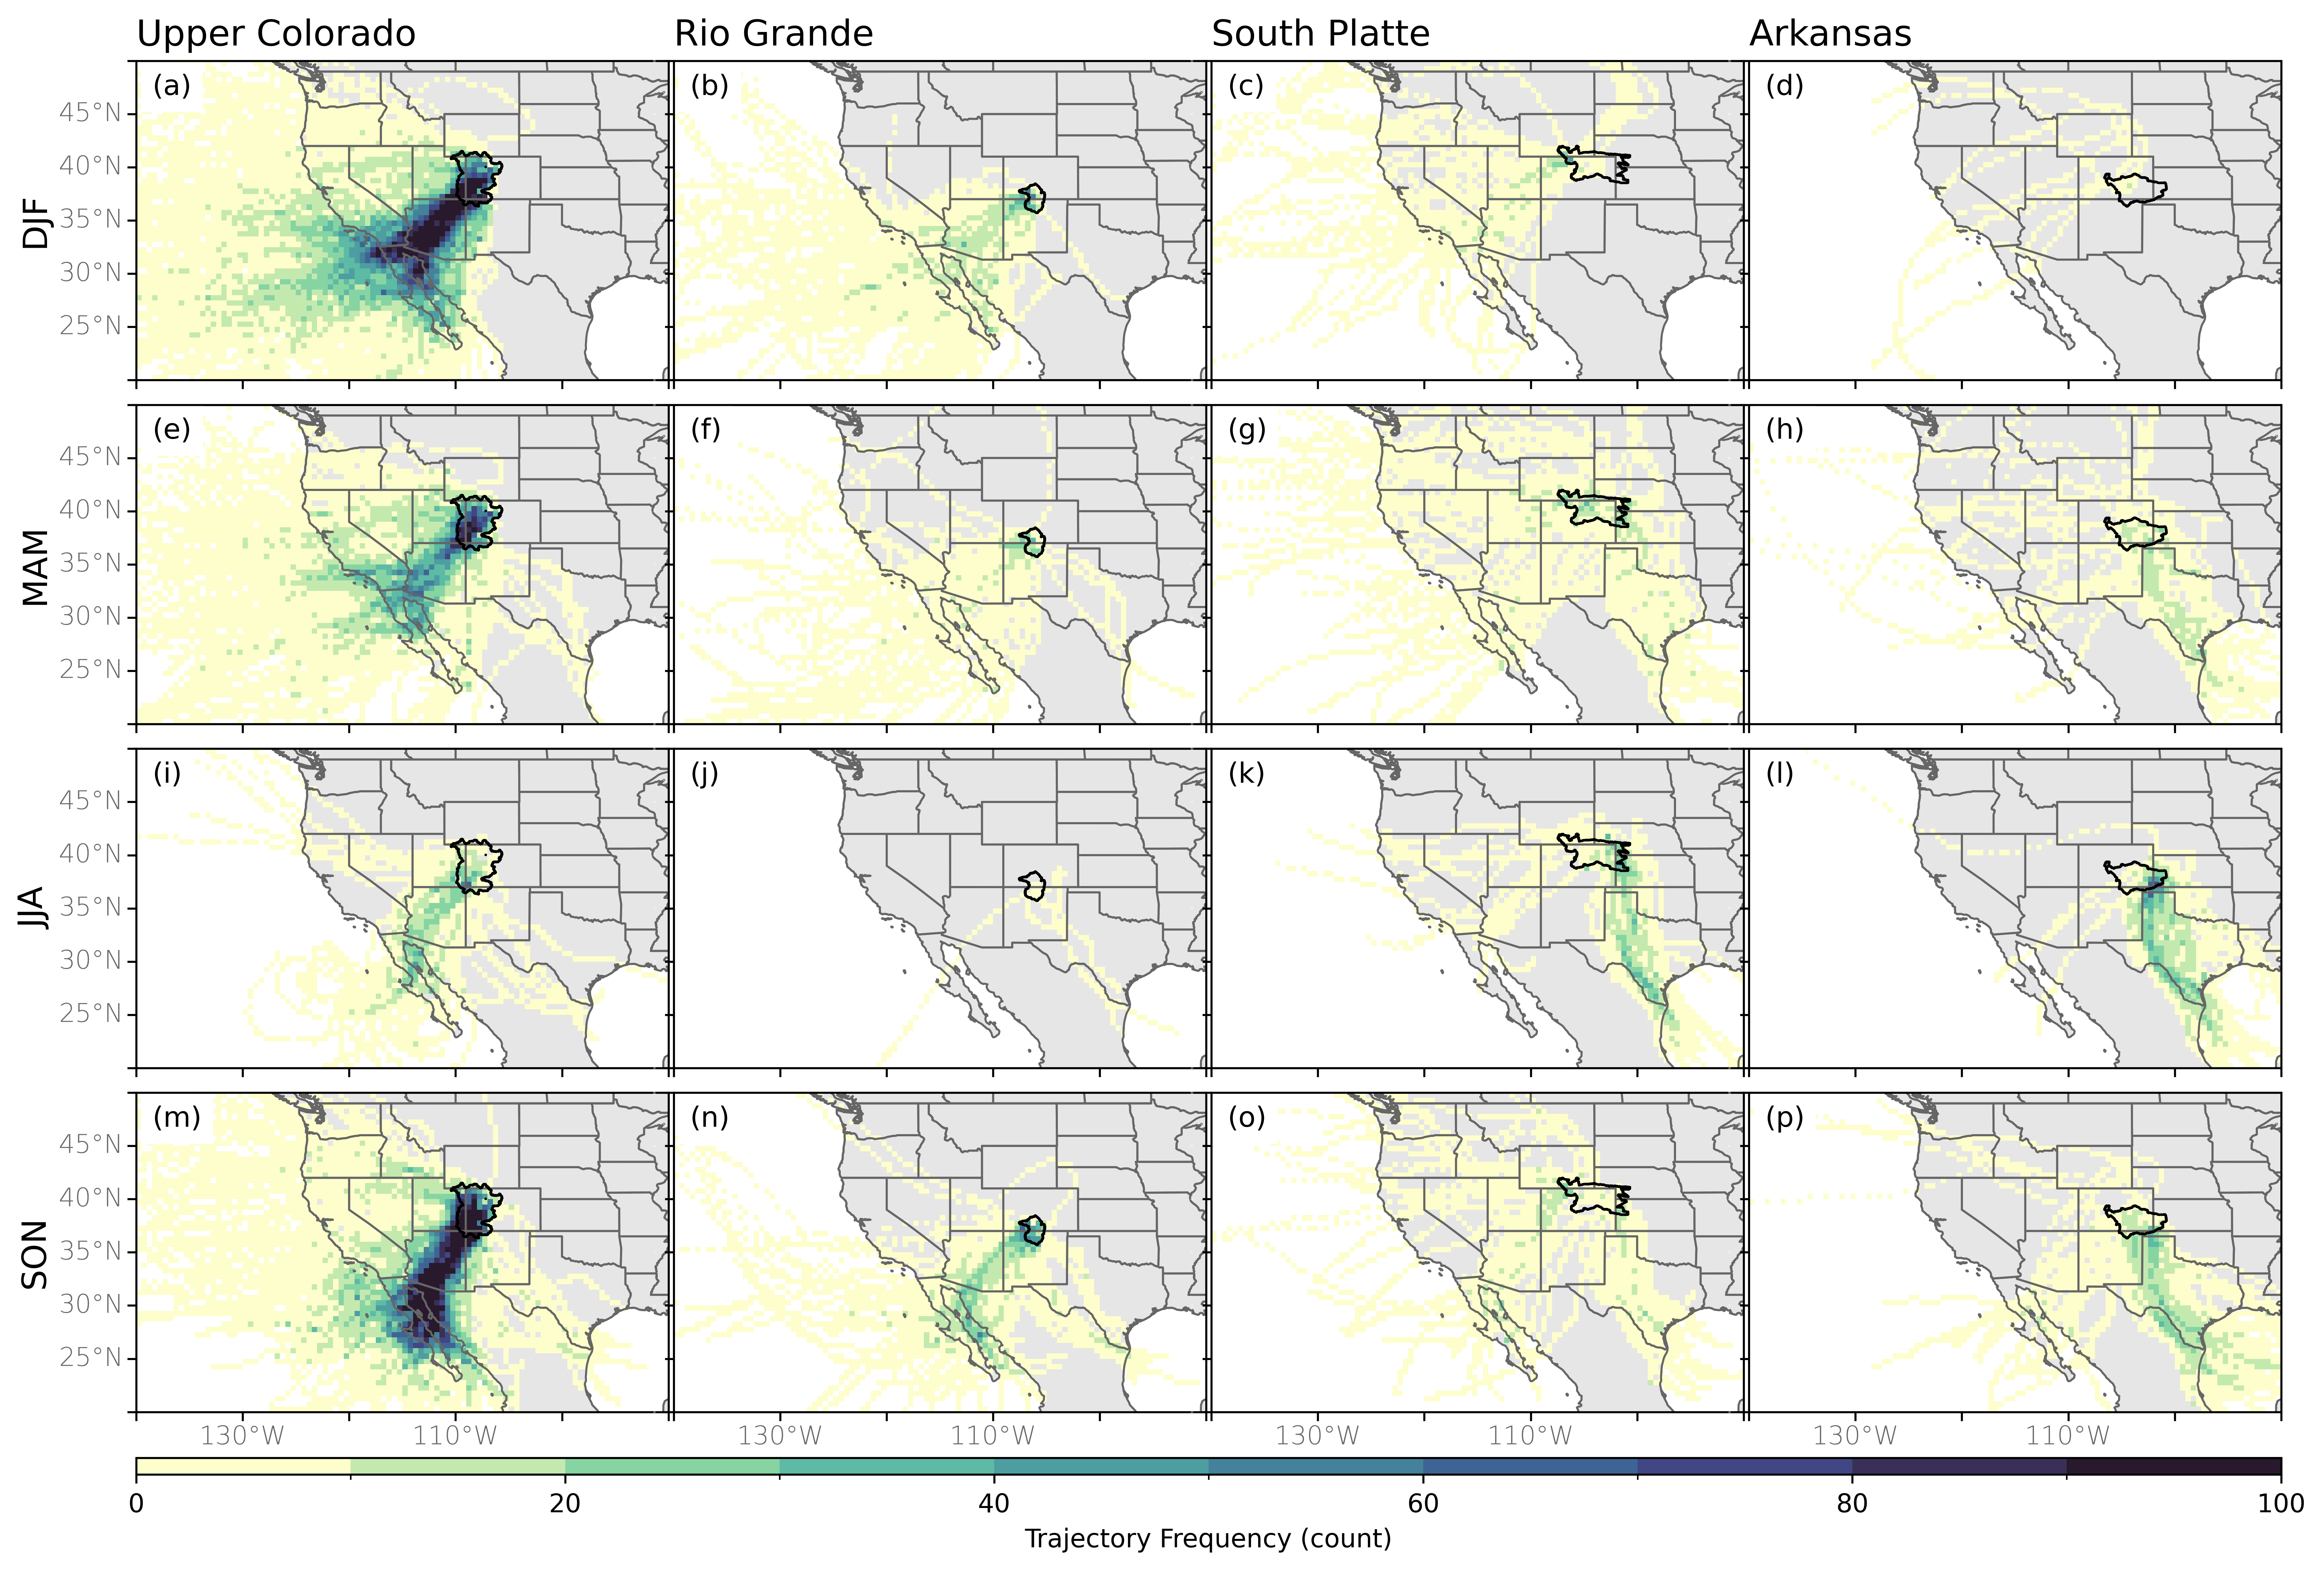
\includegraphics[width=\textwidth]{figS3.png}
\caption{(a) The trajectory frequency (shading; count) for all Colorado subbasins that fall within the Colorado region (black contour) for the months of November to April from 2000 to 2023. (b) Same as (a) but for the Rio Grande region. (c) Same as (a) but for the South Platte region. (d) Same as (a) but for the Arkansas region. (e) Same as (a) but for the months of March to May. (f) Same as (e) but for the Rio Grande region. (g) Same as (e) but for the South Platte region. (h) Same as (e) but for the Arkansas region. (i) Same as (a) but for the months of June to August. (j) Same as (i) but for the Rio Grande region. (k) Same as (i) but for the South Platte region. (l) Same as (i) but for the Arkansas region. (m) Same as (a) but for the months of September to October. (n) Same as (m) but for the Rio Grande region. (o) Same as (m) but for the South Platte region. (p) Same as (m) but for the Arkansas region.}
\label{fig:supp:spaghetti_ssn}
\end{figure}

\begin{figure}
\noindent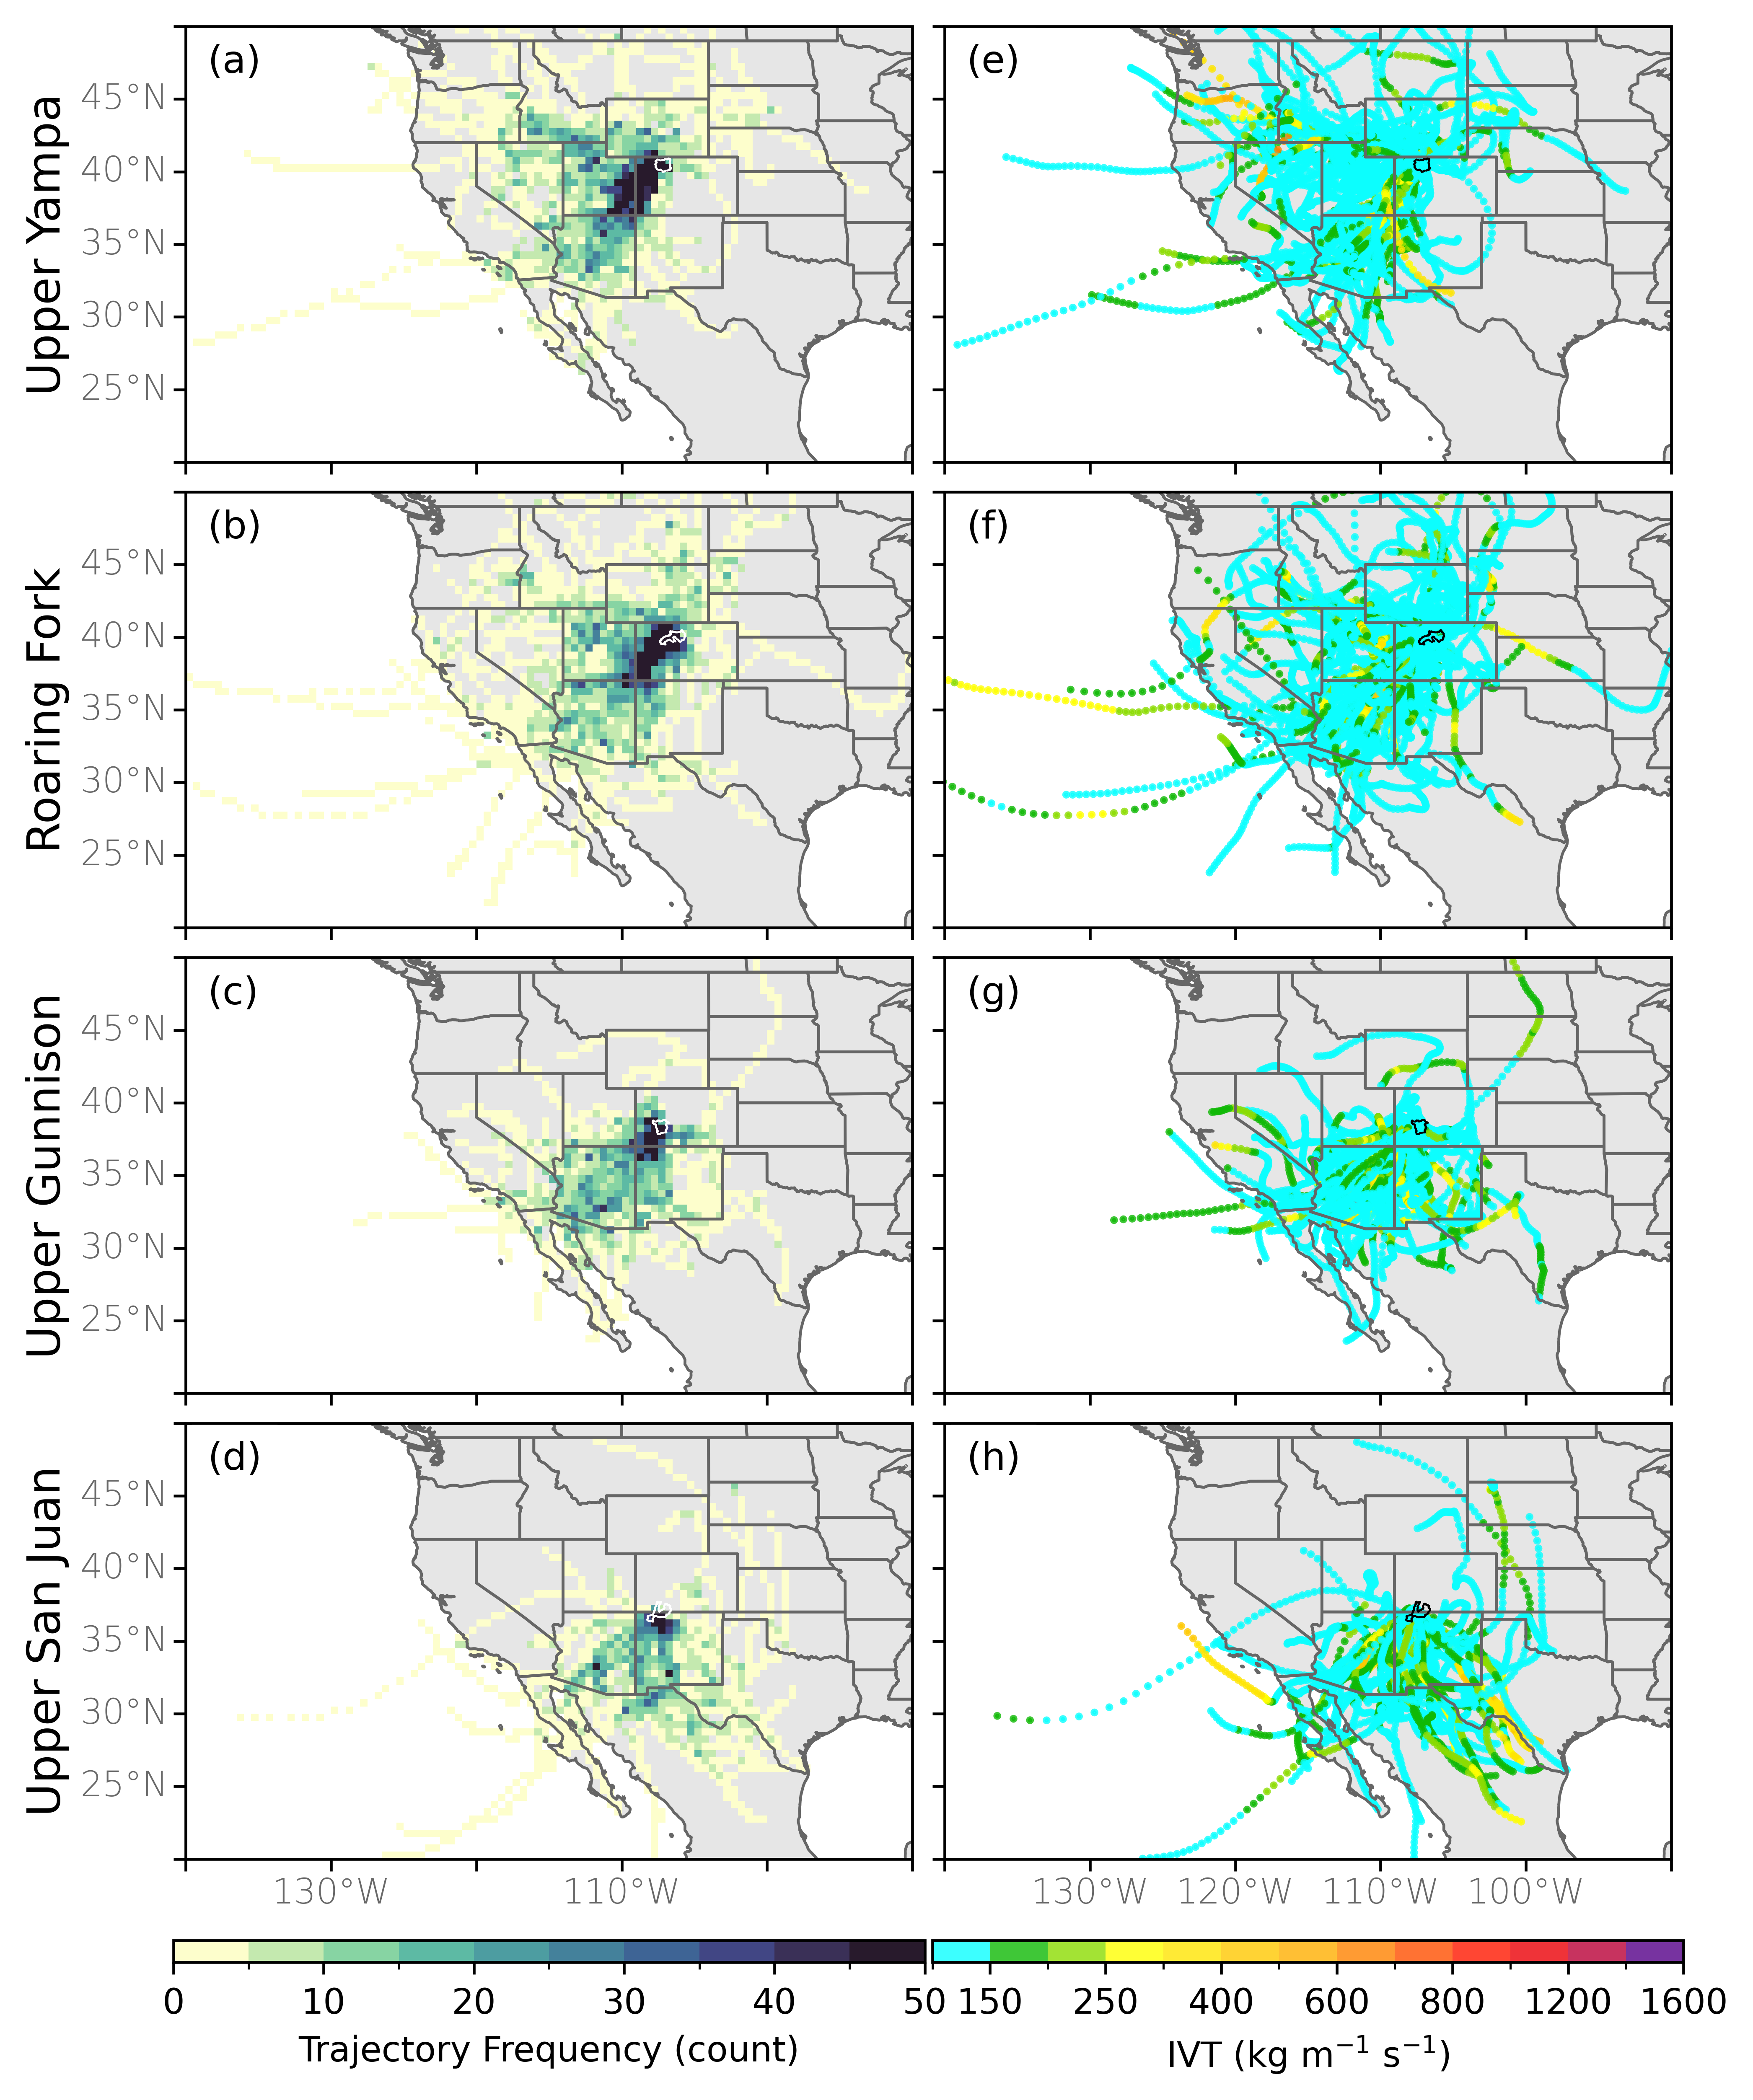
\includegraphics[width=\textwidth]{figS4.png}
\caption{(a,c,e) Daily average composites of NDJFMA IVT (shaded and vectors; kg m\textsuperscript{-1} s\textsuperscript{-1}) and 700 hPa geopotential heights (contours; m) for 24 hours after trajectories associated with an AR at the coast fall within the red bounding box. The number of trajectories is identified in the upper left corner. (b,d,f) Daily average anomaly composites of NDJFMA IVT (shaded and vectors; kg m\textsuperscript{-1} s\textsuperscript{-1}) and 700 hPa geopotential heights (contours; m) for 24 hours after trajectories associated with an AR at the coast fall within the red bounding box. Values that are considered statistically significant at the 95\% confidence interval are indicated by the IVT vectors.}
\label{fig:supp:composites_NDJFMA_lag1}
\end{figure}

\begin{figure}
\noindent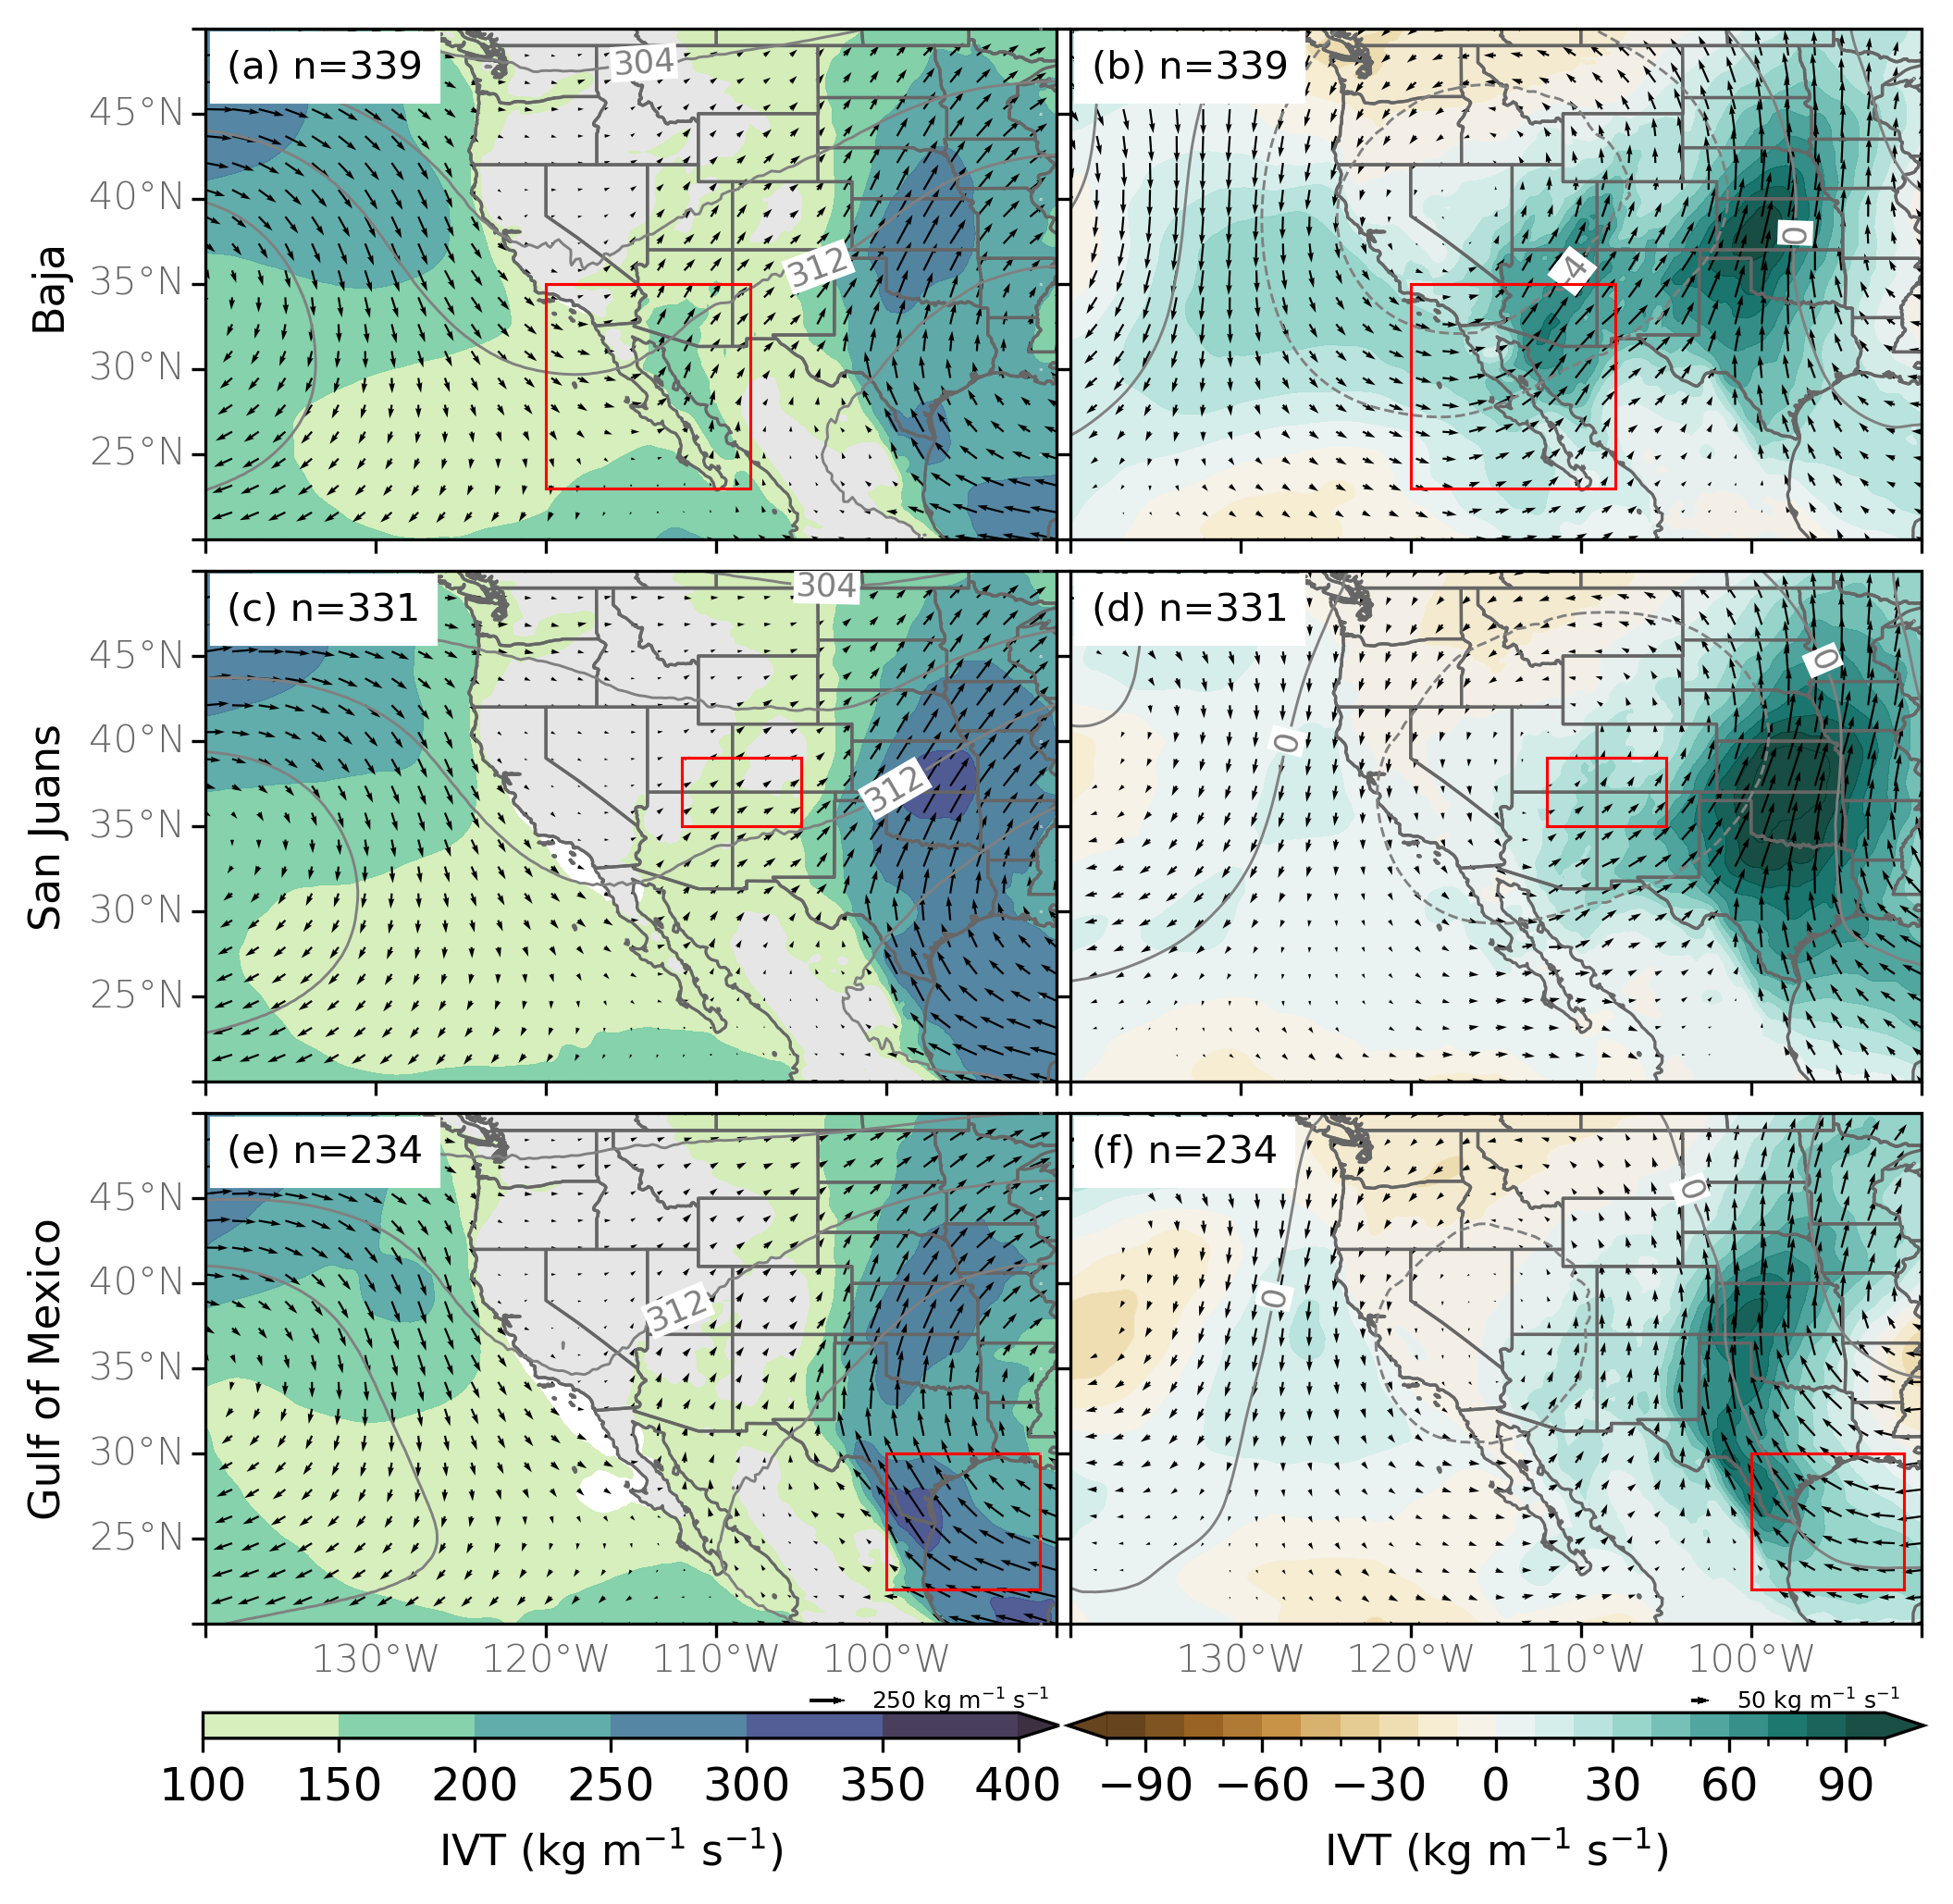
\includegraphics[width=\textwidth]{figS5.png}
\caption{Same as Fig. \ref{fig:supp:composites_NDJFMA_lag1}, but for MJJASO.}
\label{fig:supp:composites_MJJASO_lag1}
\end{figure}

\begin{figure}
\noindent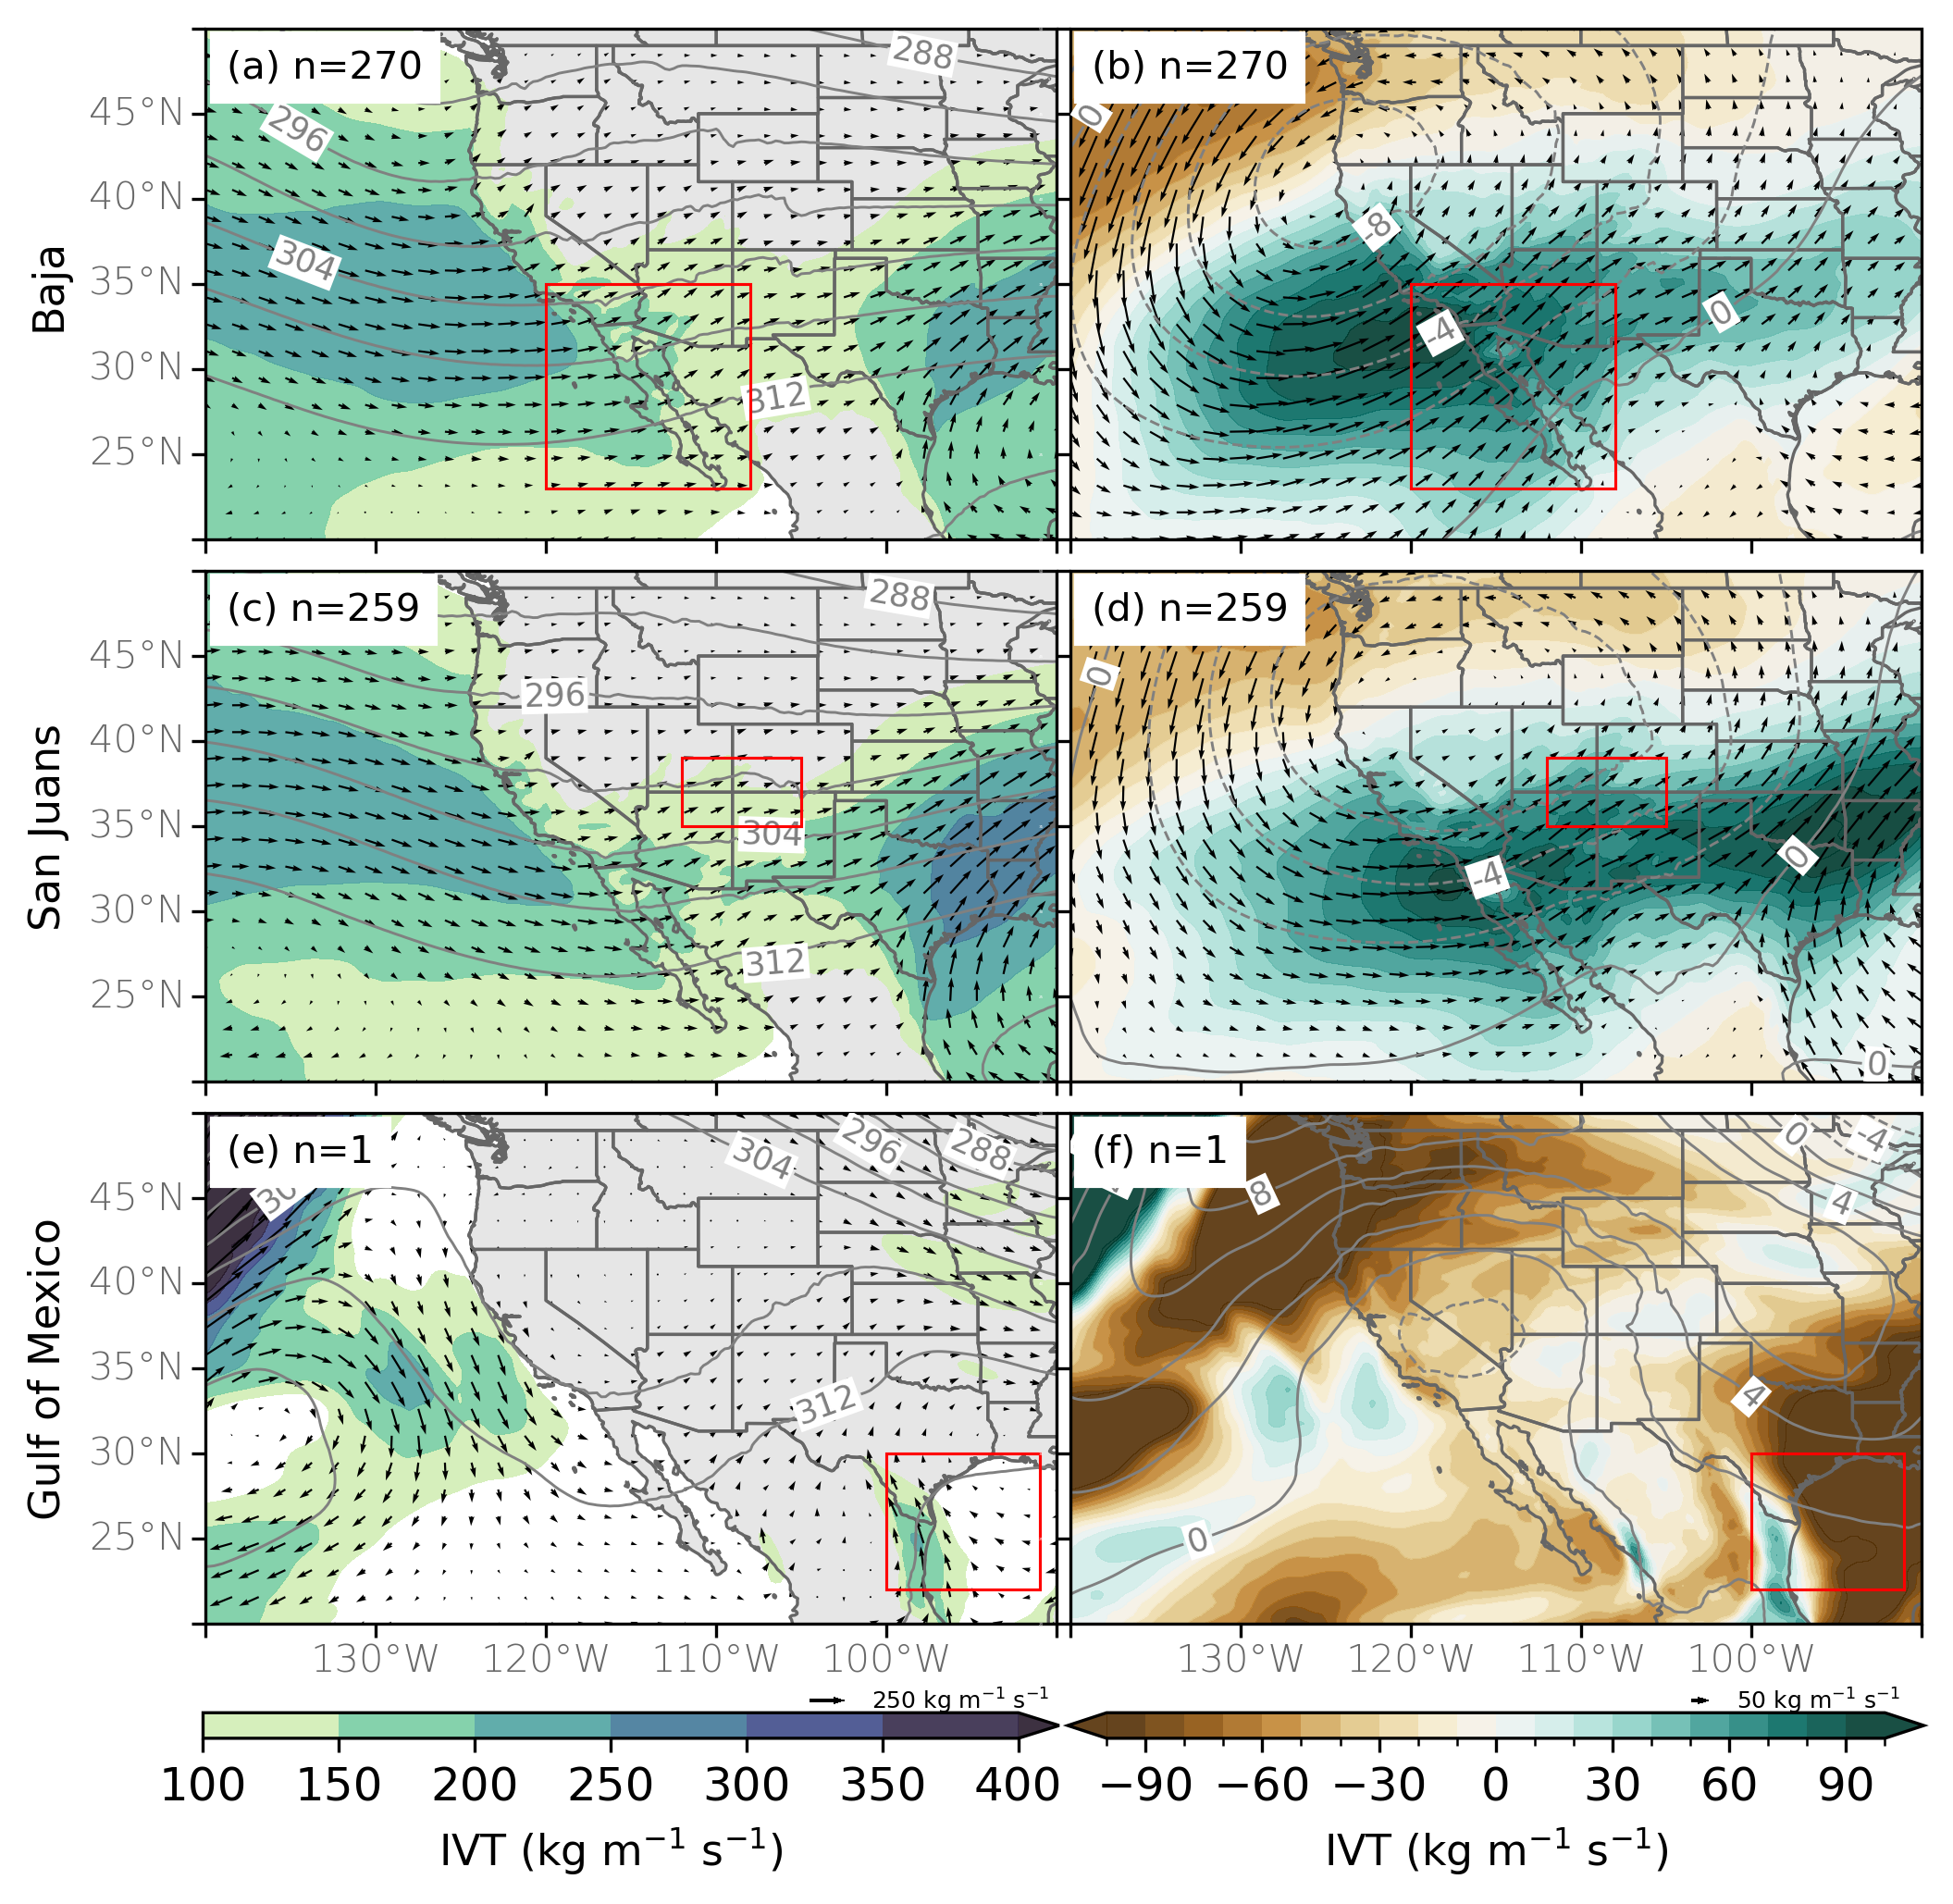
\includegraphics[width=\textwidth]{figS6.png}
\caption{(a,c,e) Daily average composites of DJF IVT (shaded and vectors; kg m\textsuperscript{-1} s\textsuperscript{-1}) and 700 hPa geopotential heights (contours; m) for days when trajectories associated with an AR at the coast fall within the red bounding box. The number of trajectories is identified in the upper left corner. (b,d,f) Daily average anomaly composites of DJF IVT (shaded and vectors; kg m\textsuperscript{-1} s\textsuperscript{-1}) and 700 hPa geopotential heights (contours; m) for days when trajectories associated with an AR at the coast fall within the red bounding box. Values that are considered statistically significant at the 95\% confidence interval are indicated by the IVT vectors.}
\label{fig:supp:composites_DJF}
\end{figure}

\begin{figure}
\noindent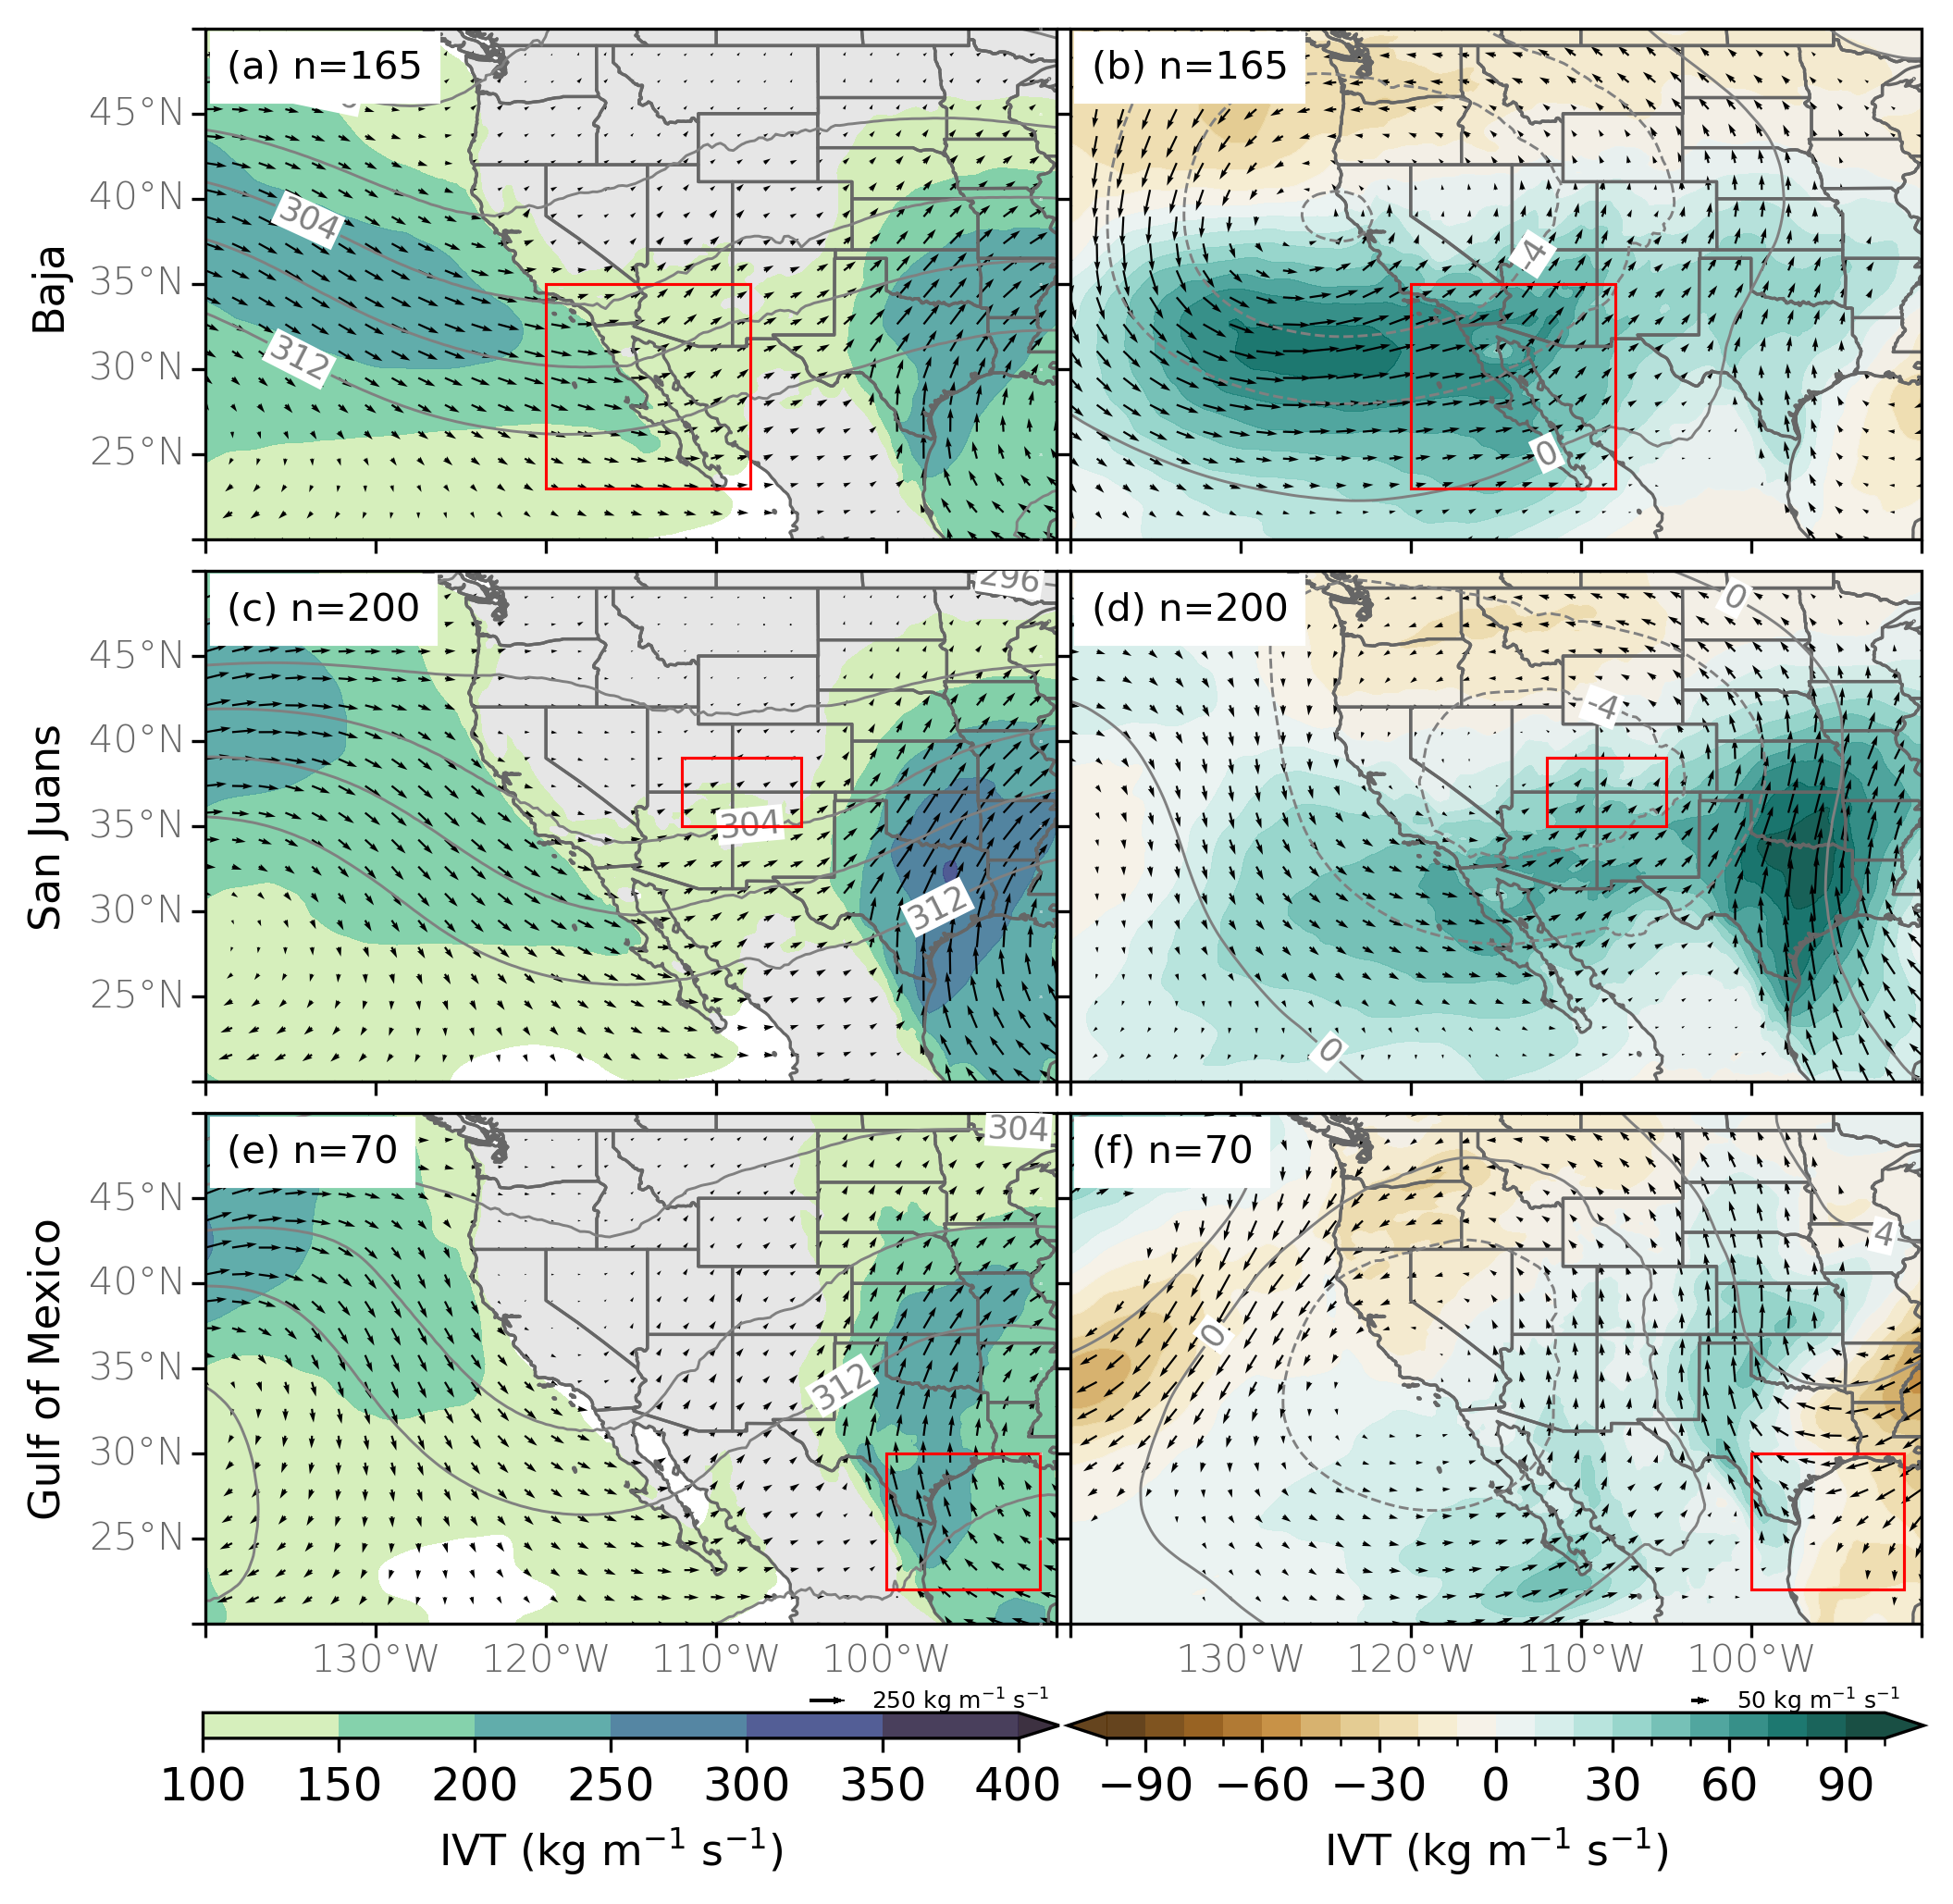
\includegraphics[width=\textwidth]{figS7.png}
\caption{Same as Fig. \ref{fig:supp:composites_DJF}, but for MAM.}
\label{fig:supp:composites_MAM}
\end{figure}

\begin{figure}
\noindent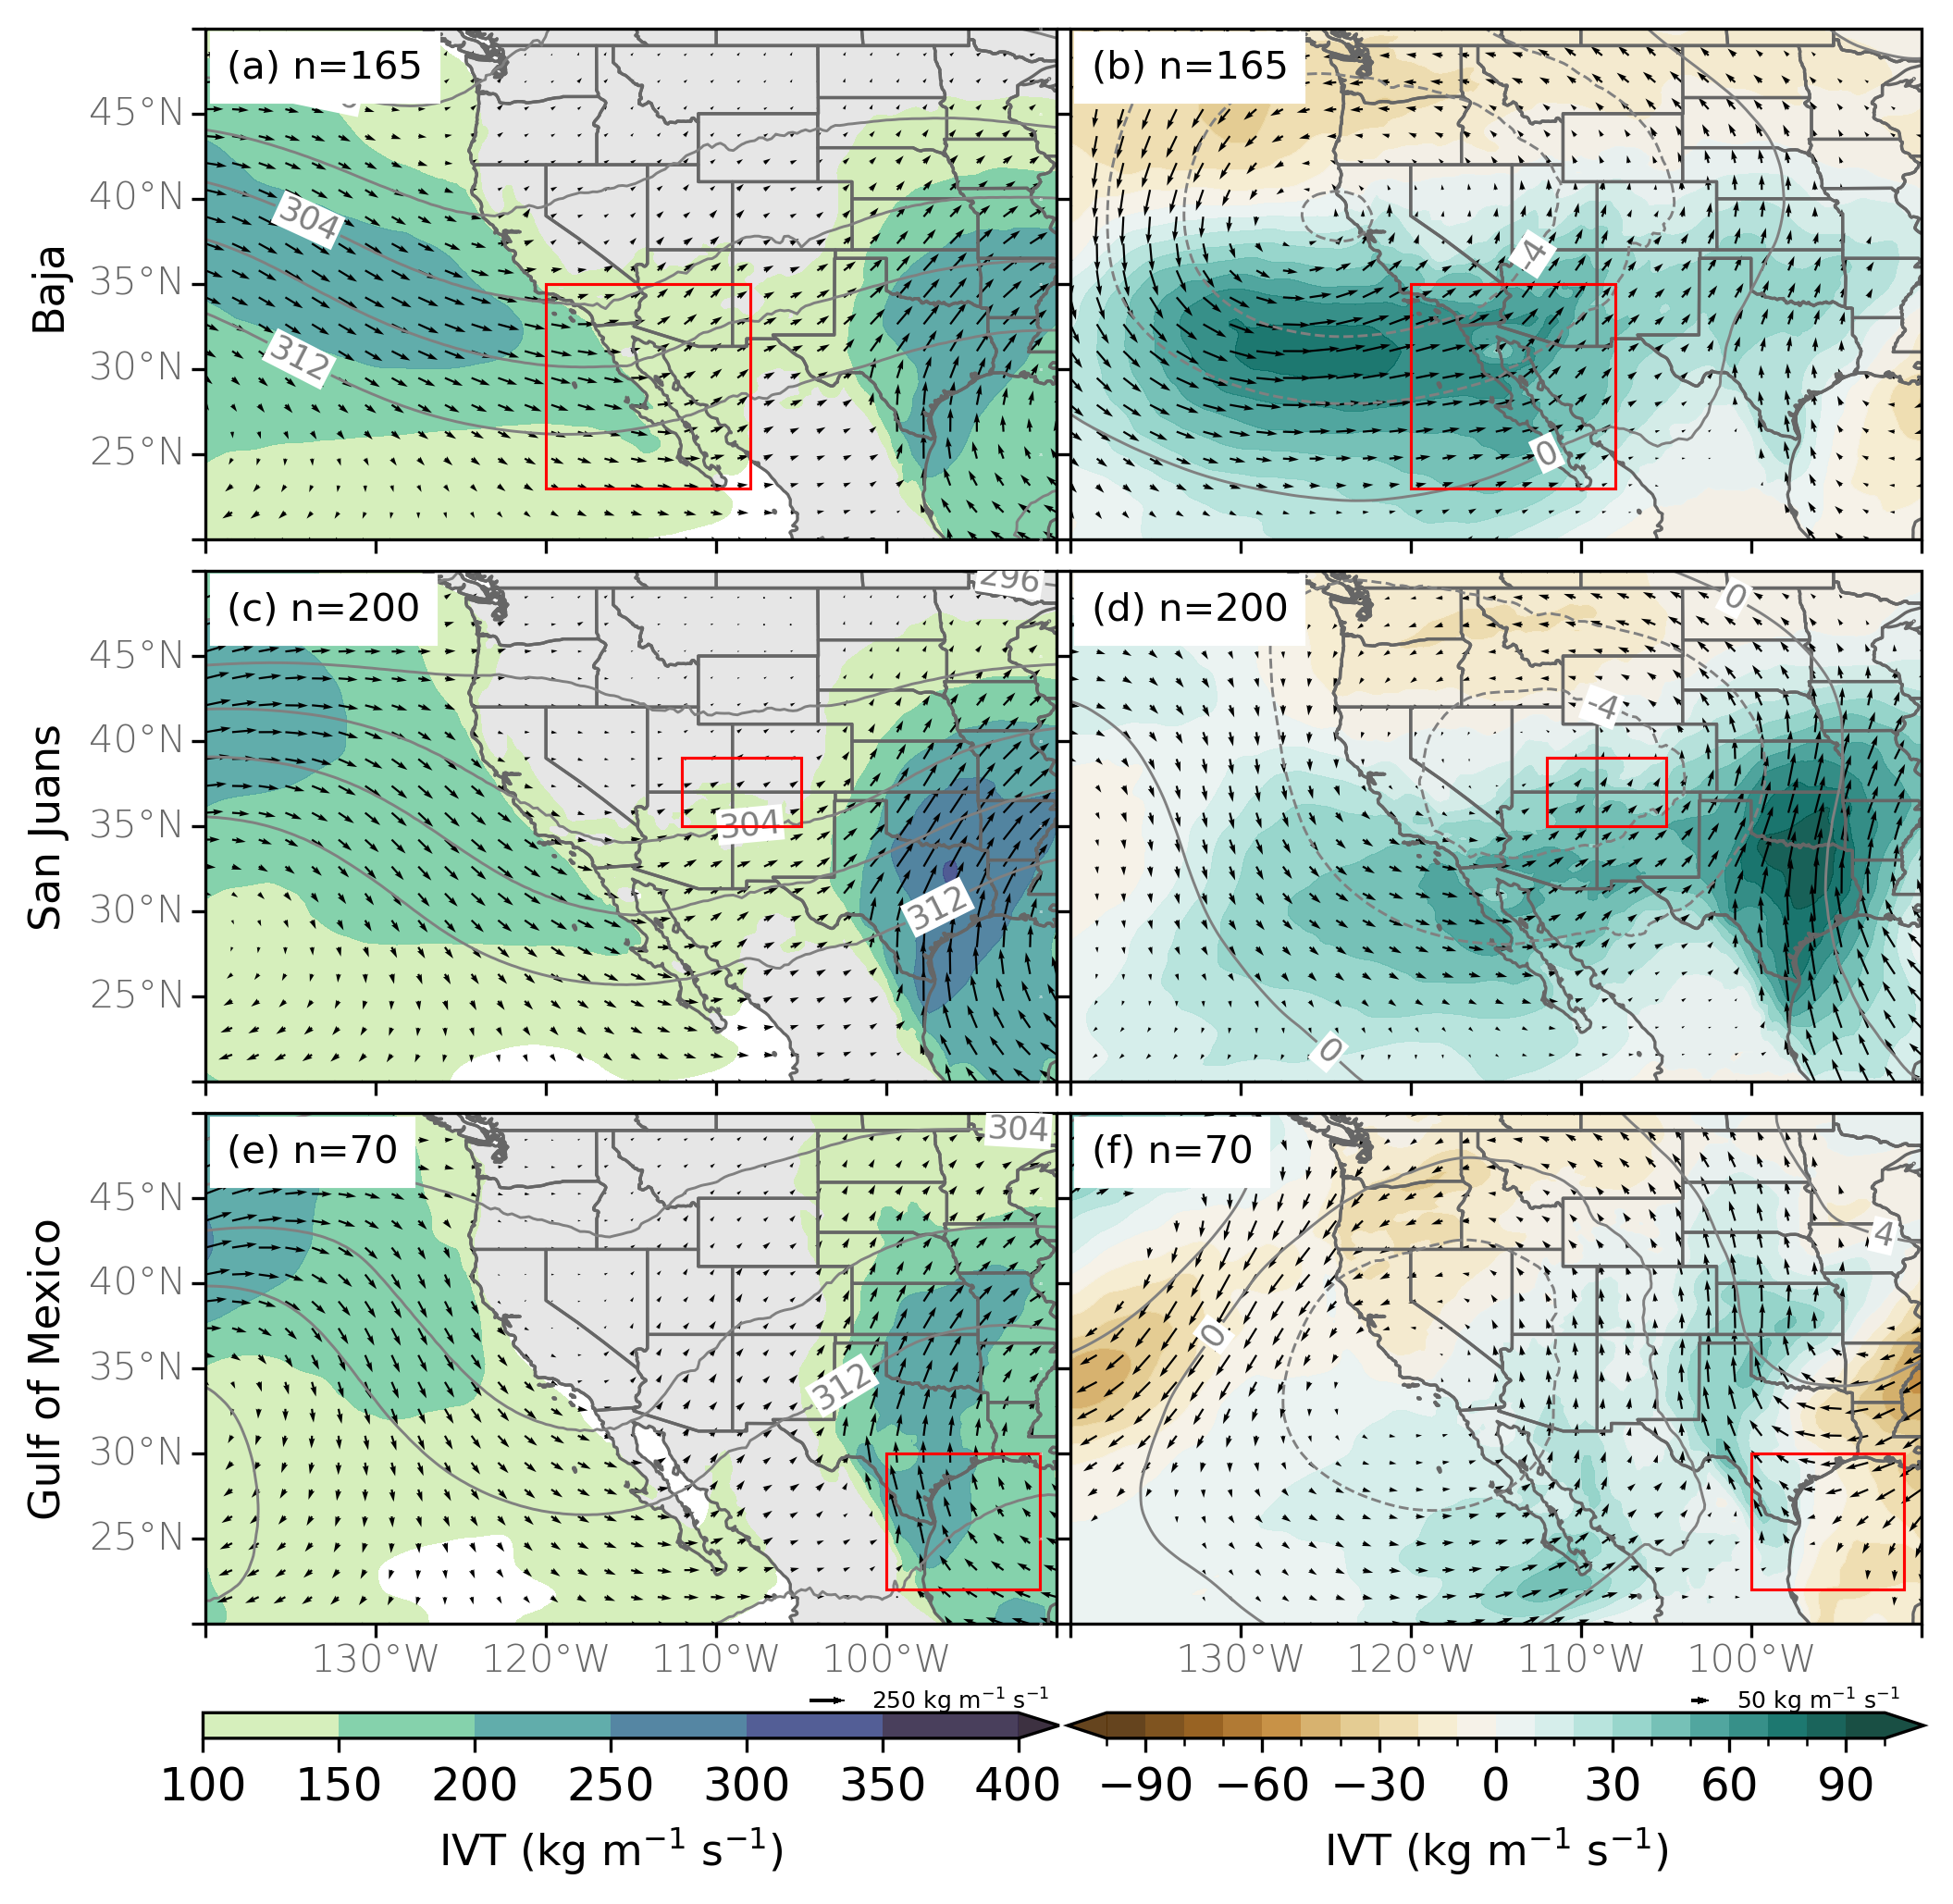
\includegraphics[width=\textwidth]{figS8.png}
\caption{Same as Fig. \ref{fig:supp:composites_DJF}, but for JJA.}
\label{fig:supp:composites_JJA}
\end{figure}

\begin{figure}
\noindent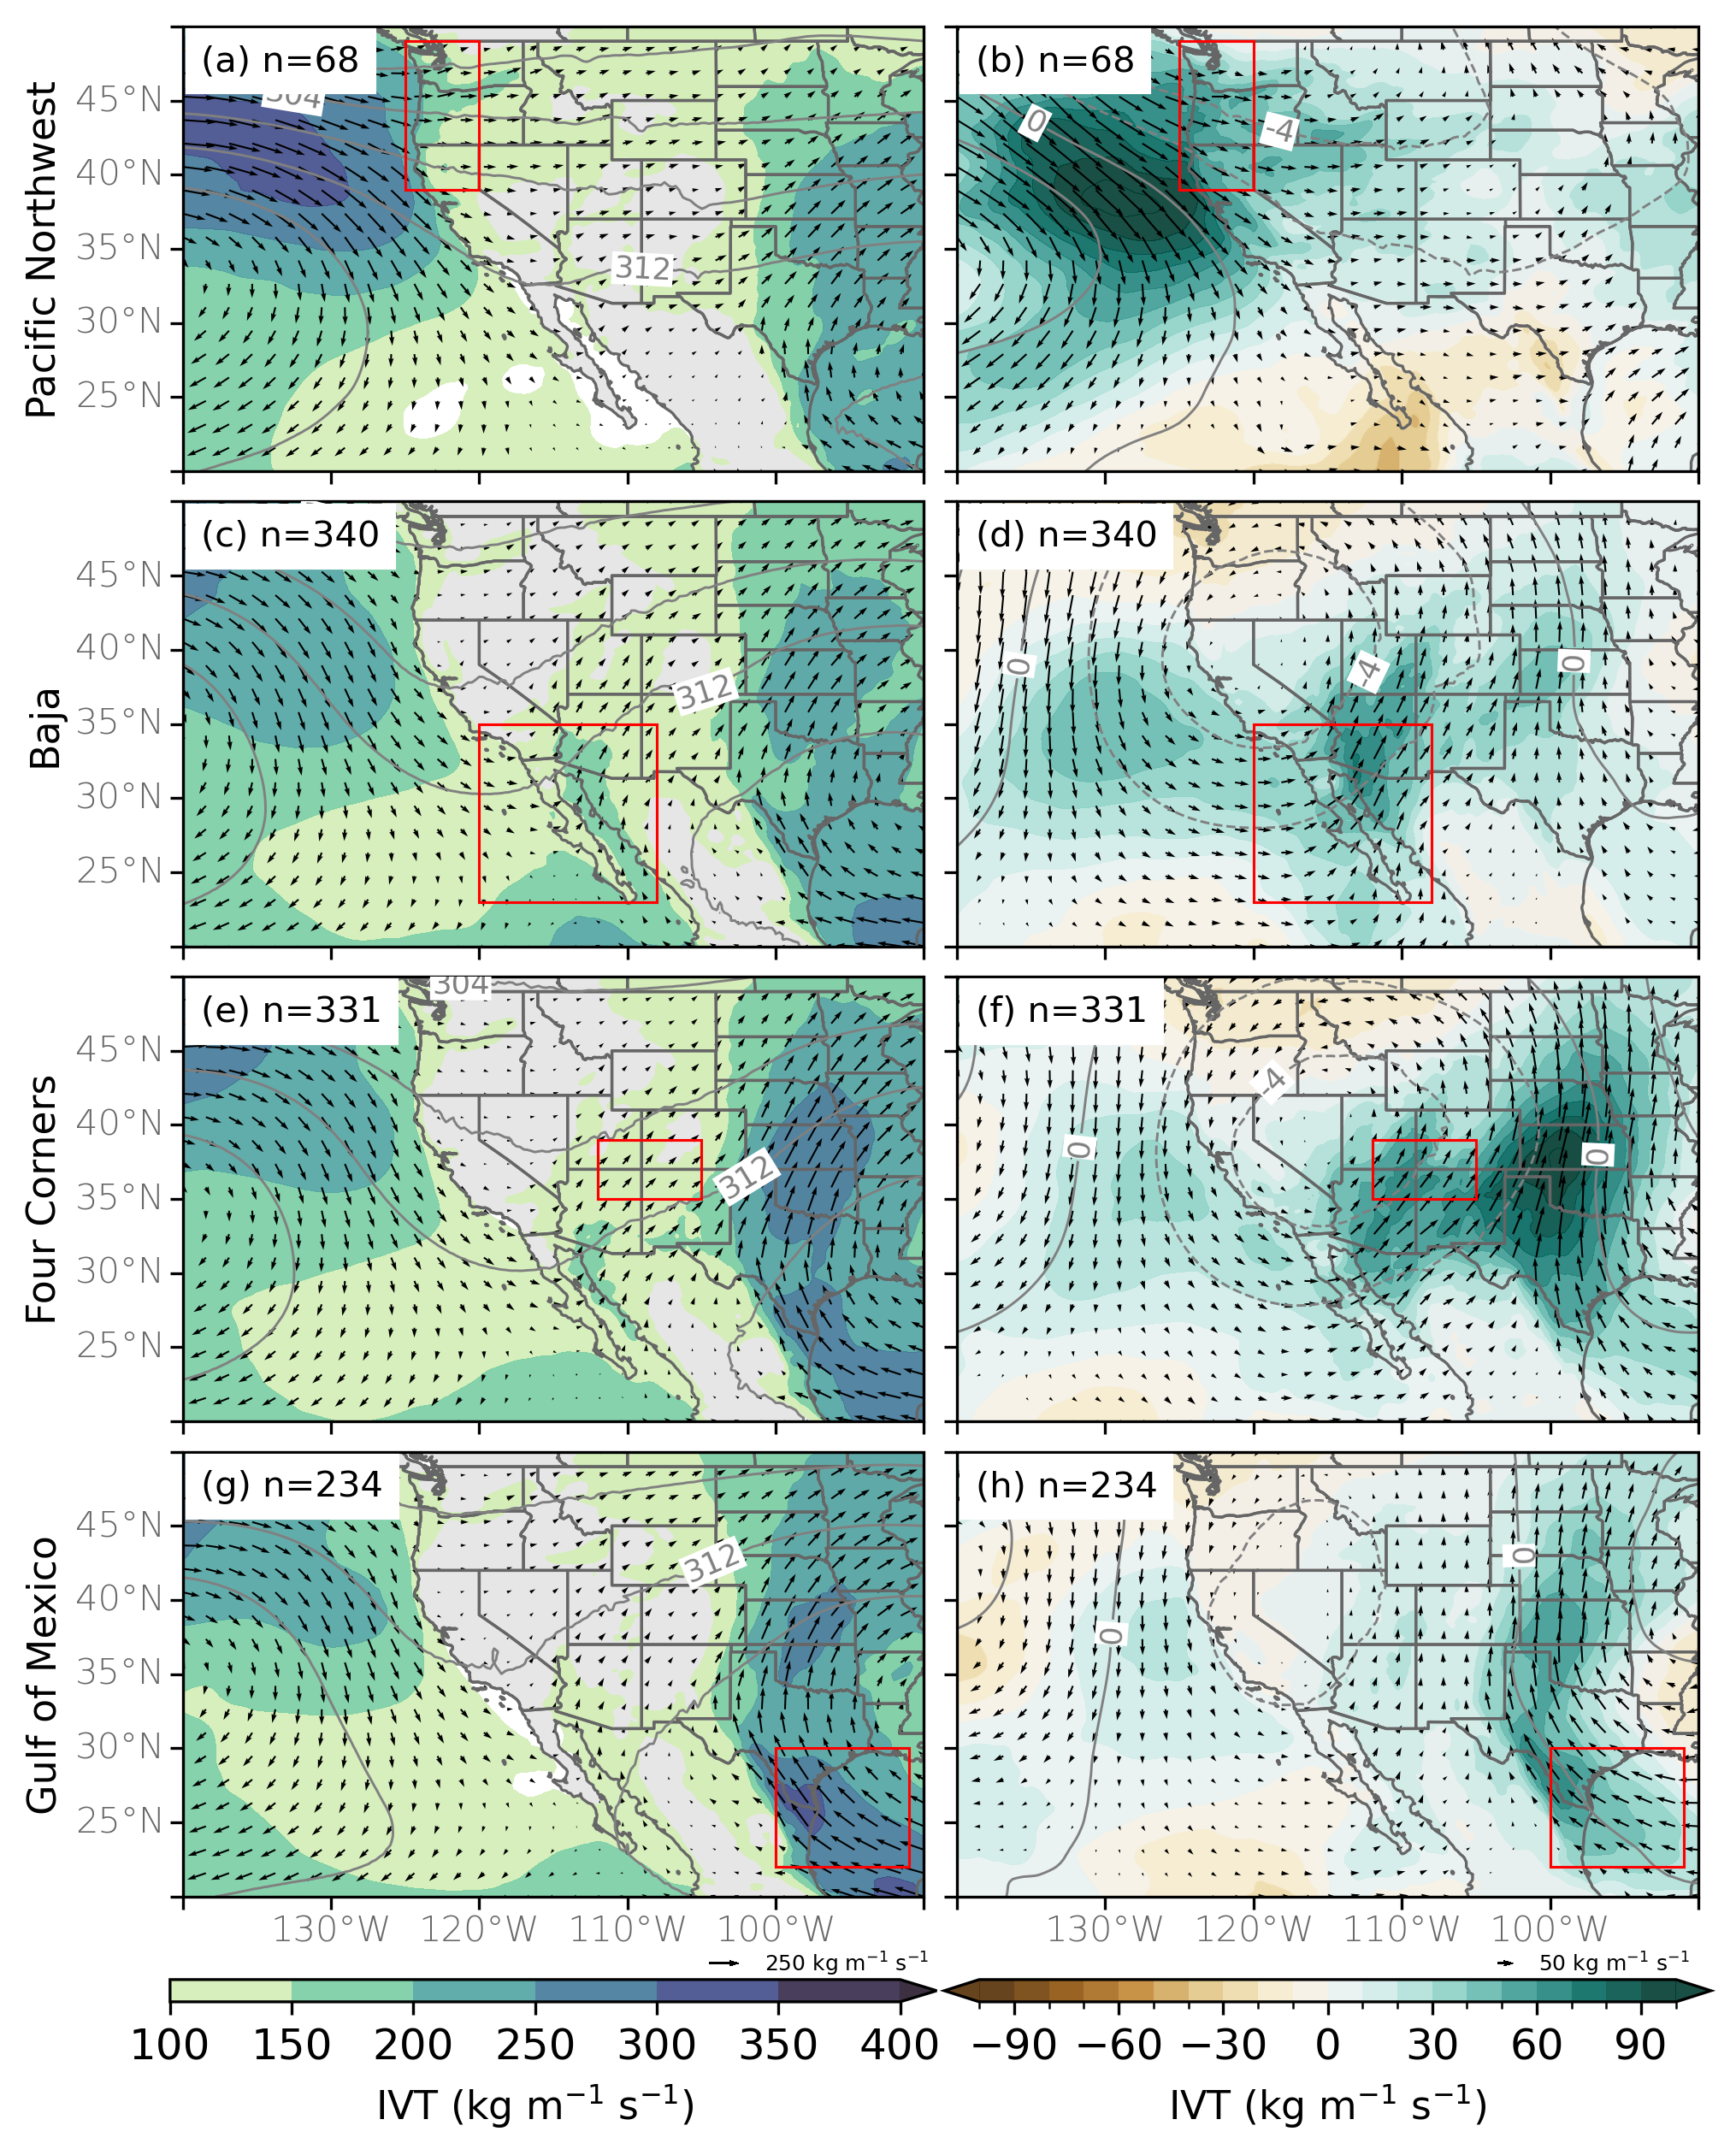
\includegraphics[width=\textwidth]{figS9.png}
\caption{Same as Fig. \ref{fig:supp:composites_DJF}, but for SON.}
\label{fig:supp:composites_SON}
\end{figure}



%Delete all unused file types below. Copy/paste for multiples of each file type as needed.
% \noindent\textbf{Text S1.}
%Type or paste text here. This should be additional explanatory text, such as: extended descriptions of results, full details of models, extended lists of acknowledgements etc.  It should not be additional discussion, analysis, interpretation or critique. It should not be an additional scientific experiment or paper.
%
%Repeat for any additional Supporting Text

%%Enter Data Set, Movie, and Audio captions here
%%EXAMPLE CAPTIONS

% \noindent\textbf{Data Set S1.} %Type or paste caption here.
%upload your dataset(s) to AGU's journal submission site and select "Supporting Information (SI)" as the file type. Following naming %convention: ds01.

%Repeat for any additional Supporting data sets

% \noindent\textbf{Movie S1.} %Type or paste caption here.
%upload your movie(s) to AGU's journal submission site and select, "Supporting Information %(SI)" as the file type. Following naming convention: ms01.

%Repeat any additional Supporting movies

% \noindent\textbf{Audio S1.} %Type or paste caption here.
%upload your audio file(s) to AGU's journal submission site and select "Supporting Information %(SI)" as the file type. Following naming convention: auds01.


%Repeat for any additional Supporting audio files

%%% End of body of article:
%%%%%%%%%%%%%%%%%%%%%%%%%%%%%%%%%%%%%%%%%%%%%%%%%%%%%%%%%%%%%%%%
%
% Optional Notation section goes here
%
% Notation -- End each entry with a period.
% \begin{notation}
% Term & definition.\\
% Second term & second definition.\\
% \end{notation}
%%%%%%%%%%%%%%%%%%%%%%%%%%%%%%%%%%%%%%%%%%%%%%%%%%%%%%%%%%%%%%%%


%% ------------------------------------------------------------------------ %%
%%  REFERENCE LIST AND TEXT CITATIONS

%%%%%%%%%%%%%%%%%%%%%%%%%%%%%%%%%%%%%%%%%%%%%%%
% 
%
% \bibliography{<name of your .bib file>} do not specify file extension
%
% no need to specify bibliographystyle
%
% Note that ALL references in this supporting information file must also be referenced in the primary manuscript
%
%%%%%%%%%%%%%%%%%%%%%%%%%%%%%%%%%%%%%%%%%%%%%%%
% if you get an error about newblock being undefined, uncomment this line:
%\newcommand{\newblock}{}

% \bibliography{ uncomment this line and enter the name of your bibtex file here } 




%Reference citation instructions and examples:
%
% Please use ONLY \cite and \citeA for reference citations.
% \cite for parenthetical references
% ...as shown in recent studies (Simpson et al., 2019)
% \citeA for in-text citations
% ...Simpson et al (2019) have shown...
% DO NOT use other cite commands (e.g., \citet, \citep, \citeyear, \nocite, \citealp, etc.).
%
%
%...as shown by \citeA{jskilby}.
%...as shown by \citeA{lewin76}, \citeA{carson86}, \citeA{bartoldy02}, and \citeA{rinaldi03}.
%...has been shown \cite<e.g.,>{jskilbye}.
%...has been shown \cite{lewin76,carson86,bartoldy02,rinaldi03}.
%...has been shown \cite{lewin76,carson86,bartoldy02,rinaldi03}.
%
% apacite uses < > for prenotes, not [ ]
% DO NOT use other cite commands (e.g., \citet, \citep, \citeyear, \nocite, \citealp, etc.).
%

%% ------------------------------------------------------------------------ %%
%
%  END ARTICLE
%
%% ------------------------------------------------------------------------ %%
% \end{article}


% Copy/paste for multiples of each file type as needed.

% enter figures and tables below here: %%%%%%%
%
%
%
%
% EXAMPLE FIGURES
% ---------------
% If you get an error about an unknown bounding box, try specifying the width and height of the figure with the natwidth and natheight options.
% \begin{figure}
%\setfigurenum{S1} %%You can change number for each figure if you want, not required. "S" prepended automatically.
% \noindent\includegraphics[natwidth=800px,natheight=600px]{samplefigure.eps}
%\caption{caption}
%\label{epsfiguresample}
%\end{figure}
%
%
% Giving latex a width will help it to scale the figure properly. A simple trick is to use \textwidth. Try this if large figures run off the side of the page.
% \begin{figure}
% \noindent\includegraphics[width=\textwidth]{anothersample.png}
%\caption{caption}
%\label{pngfiguresample}
%\end{figure}
%
%
%\begin{figure}
%\noindent\includegraphics[width=\textwidth]{athirdsample.pdf}
%\caption{A pdf test figure}
%\label{pdffiguresample}
%\end{figure}
%
% PDFLatex does not seem to be able to process EPS figures. You may want to try the epstopdf package.
%
%
% ---------------
% EXAMPLE TABLE
%
%\begin{table}
%\settablenum{S1} %%Change number for each table
%\caption{Time of the Transition Between Phase 1 and Phase 2\tablenotemark{a}}
%\centering
%\begin{tabular}{l c}
%\hline
% Run  & Time (min)  \\
%\hline
%  $l1$  & 260   \\
%  $l2$  & 300   \\
%  $l3$  & 340   \\
%  $h1$  & 270   \\
%  $h2$  & 250   \\
%  $h3$  & 380   \\
%  $r1$  & 370   \\
%  $r2$  & 390   \\
%\hline
%\end{tabular}
%\tablenotetext{a}{Footnote text here.}
%\end{table}
% ---------------
%
% EXAMPLE LARGE TABLE (UPLOADED SEPARATELY)
%\begin{table}
%\settablenum{S1} %%Change number for each table
%\caption{Time of the Transition Between Phase 1 and Phase 2\tablenotemark{a}}
%\end{table}


\end{document}

%%%%%%%%%%%%%%%%%%%%%%%%%%%%%%%%%%%%%%%%%%%%%%%%%%%%%%%%%%%%%%%

More Information and Advice:

%% ------------------------------------------------------------------------ %%
%
%  SECTION HEADS
%
%% ------------------------------------------------------------------------ %%

% Capitalize the first letter of each word (except for
% prepositions, conjunctions, and articles that are
% three or fewer letters).

% AGU follows standard outline style; therefore, there cannot be a section 1 without
% a section 2, or a section 2.3.1 without a section 2.3.2.
% Please make sure your section numbers are balanced.
% ---------------
% Level 1 head
%
% Use the \section{} command to identify level 1 heads;
% type the appropriate head wording between the curly
% brackets, as shown below.
%
%An example:
%\section{Level 1 Head: Introduction}
%
% ---------------
% Level 2 head
%
% Use the \subsection{} command to identify level 2 heads.
%An example:
%\subsection{Level 2 Head}
%
% ---------------
% Level 3 head
%
% Use the \subsubsection{} command to identify level 3 heads
%An example:
%\subsubsection{Level 3 Head}
%
%---------------
% Level 4 head
%
% Use the \subsubsubsection{} command to identify level 3 heads
% An example:
%\subsubsubsection{Level 4 Head} An example.
%
%% ------------------------------------------------------------------------ %%
%
%  IN-TEXT LISTS
%
%% ------------------------------------------------------------------------ %%
%
% Do not use bulleted lists; enumerated lists are okay.
% \begin{enumerate}
% \item
% \item
% \item
% \end{enumerate}
%
%% ------------------------------------------------------------------------ %%
%
%  EQUATIONS
%
%% ------------------------------------------------------------------------ %%

% Single-line equations are centered.
% Equation arrays will appear left-aligned.

Math coded inside display math mode \[ ...\]
 will not be numbered, e.g.,:
 \[ x^2=y^2 + z^2\]

 Math coded inside \begin{equation} and \end{equation} will
 be automatically numbered, e.g.,:
 \begin{equation}
 x^2=y^2 + z^2
 \end{equation}

% IF YOU HAVE MULTI-LINE EQUATIONS, PLEASE
% BREAK THE EQUATIONS INTO TWO OR MORE LINES
% OF SINGLE COLUMN WIDTH (20 pc, 8.3 cm)
% using double backslashes (\\).

% To create multiline equations, use the
% \begin{eqnarray} and \end{eqnarray} environment
% as demonstrated below.
\begin{eqnarray}
  x_{1} & = & (x - x_{0}) \cos \Theta \nonumber \\
        && + (y - y_{0}) \sin \Theta  \nonumber \\
  y_{1} & = & -(x - x_{0}) \sin \Theta \nonumber \\
        && + (y - y_{0}) \cos \Theta.
\end{eqnarray}

%If you don't want an equation number, use the star form:
%\begin{eqnarray*}...\end{eqnarray*}

% Break each line at a sign of operation
% (+, -, etc.) if possible, with the sign of operation
% on the new line.

% Indent second and subsequent lines to align with
% the first character following the equal sign on the
% first line.

% Use an \hspace{} command to insert horizontal space
% into your equation if necessary. Place an appropriate
% unit of measure between the curly braces, e.g.
% \hspace{1in}; you may have to experiment to achieve
% the correct amount of space.


%% ------------------------------------------------------------------------ %%
%
%  EQUATION NUMBERING: COUNTER
%
%% ------------------------------------------------------------------------ %%

% You may change equation numbering by resetting
% the equation counter or by explicitly numbering
% an equation.

% To explicitly number an equation, type \eqnum{}
% (with the desired number between the brackets)
% after the \begin{equation} or \begin{eqnarray}
% command.  The \eqnum{} command will affect only
% the equation it appears with; LaTeX will number
% any equations appearing later in the manuscript
% according to the equation counter.
%

% If you have a multiline equation that needs only
% one equation number, use a \nonumber command in
% front of the double backslashes (\\) as shown in
% the multiline equation above.

%% ------------------------------------------------------------------------ %%
%
%  SIDEWAYS FIGURE AND TABLE EXAMPLES
%
%% ------------------------------------------------------------------------ %%
%
% For tables and figures, add \usepackage{rotating} to the paper and add the rotating.sty file to the folder.
% AGU prefers the use of {sidewaystable} over {landscapetable} as it causes fewer problems.
%
% \begin{sidewaysfigure}
% \includegraphics[width=20pc]{samplefigure.eps}
% \caption{caption here}
% \label{label_here}
% \end{sidewaysfigure}
%
%
%
% \begin{sidewaystable}
% \caption{}
% \begin{tabular}
% Table layout here.
% \end{tabular}
% \end{sidewaystable}
%
%

